\chapter{BACKGROUND AND RELATED WORKS}

% ================================================
% 1.1 Overview
% ================================================
\section{Overview}

Data quality (DQ) is a critical concern in modern data-intensive systems. As organizations increasingly rely on real-time data streams for decision-making, ensuring the quality of streaming data has become a fundamental challenge. This chapter reviews the foundational concepts, existing frameworks, and relevant datasets that form the basis of this research.

% ================================================
% 1.2 Streaming Data Processing
% ================================================
\section{Streaming Data Processing}

Streaming data processing refers to the continuous ingestion, processing, and analysis of data as it arrives, rather than in predefined batches. Key technologies in this space include Apache Kafka \citep{kafkaintro2024} for distributed event streaming, and Apache Flink \citep{flinkdocs2024} for stateful stream processing with exactly-once semantics.

\subsection{Apache Kafka: Event Streaming Platform}

According to the official Apache Kafka documentation \citep{kafkaintro2024}, Kafka is a distributed event streaming platform that combines three key capabilities: (1) publishing (write) and subscribing to (read) streams of events; (2) storing streams of events durably and reliably; and (3) processing streams of events as they occur or retrospectively. Kafka operates as a distributed system consisting of servers (brokers) and clients communicating via a high-performance TCP network protocol. Kafka is deployed on bare-metal hardware, virtual machines, containers, and in cloud environments.

The Kafka architecture centers on several core concepts \citep{kafkaintro2024}:

\begin{itemize}
    \item \textbf{Events (records/messages):} An event records the fact that ``something happened.'' Conceptually, an event has a key, value, timestamp, and optional metadata headers.
    \item \textbf{Topics:} Events are organized and durably stored in topics---similar to a folder in a filesystem, with events as files. Topics are \textit{multi-producer} and \textit{multi-subscriber}: a topic can have zero, one, or many producers writing events, and zero, one, or many consumers subscribing to events.
    \item \textbf{Partitions:} Topics are partitioned, meaning a topic is spread over a number of ``buckets'' located on different Kafka brokers. This enables both write and read parallelism across multiple brokers simultaneously. Events with the same event key are written to the same partition, guaranteeing that any consumer of a given topic-partition will always read that partition's events in exactly the same order as they were written.
    \item \textbf{Brokers:} Kafka runs as a cluster of servers forming the storage layer. Each broker holds a subset of partitions and serves as the leader for specific partitions. If any server fails, other servers take over their work to ensure continuous operations without data loss.
    \item \textbf{Producers:} Client applications that publish (write) events to Kafka, directly addressing messages to particular partitions.
    \item \textbf{Consumers:} Client applications that subscribe to (read) and process events. Kafka consumers track the maximum offset they have consumed in each partition and can commit offsets to resume from those positions after restart. Consumer groups enable parallel consumption of partitions.
    \item \textbf{Replication:} Every topic can be replicated across brokers for fault tolerance and high availability. A common production setting is a replication factor of 3.
\end{itemize}

Kafka's retention mechanism stores events durably for as long as needed (configurable per topic, e.g., 7 days). Unlike traditional messaging systems, events are not deleted after consumption. This enables replay of historical events, which is essential for backfilling baselines and reprocessing after failures. Kafka's performance remains effectively constant with respect to data size.

The Kafka Streams API \citep{kafkastreams2024} enables implementing stream processing applications and microservices with higher-level functions including transformations, stateful operations (aggregations, joins), windowing, and event-time processing. Kafka Streams partitions data for processing using the same partitioning as Kafka's storage layer, enabling data locality, elasticity, scalability, high performance, and fault tolerance.

In the context of the CA-DQStream framework, Kafka serves as the distributed event streaming backbone. NYC TLC Parquet files are ingested via Kafka Producer into the \texttt{taxi-nyc-raw} topic, and the six output/meta topics (\texttt{dq-schema-violations}, \texttt{dq-hard-rule-violations}, \texttt{dq-if-anomalies}, \texttt{dq-anomaly-scores}, \texttt{dq-meta-stream}, and \texttt{if-model-updates}) form the streaming pipeline. Figure~\ref{fig:kafka_streams_overview} shows the Kafka Streams architecture.

\begin{figure}[H]
\centering
\fbox{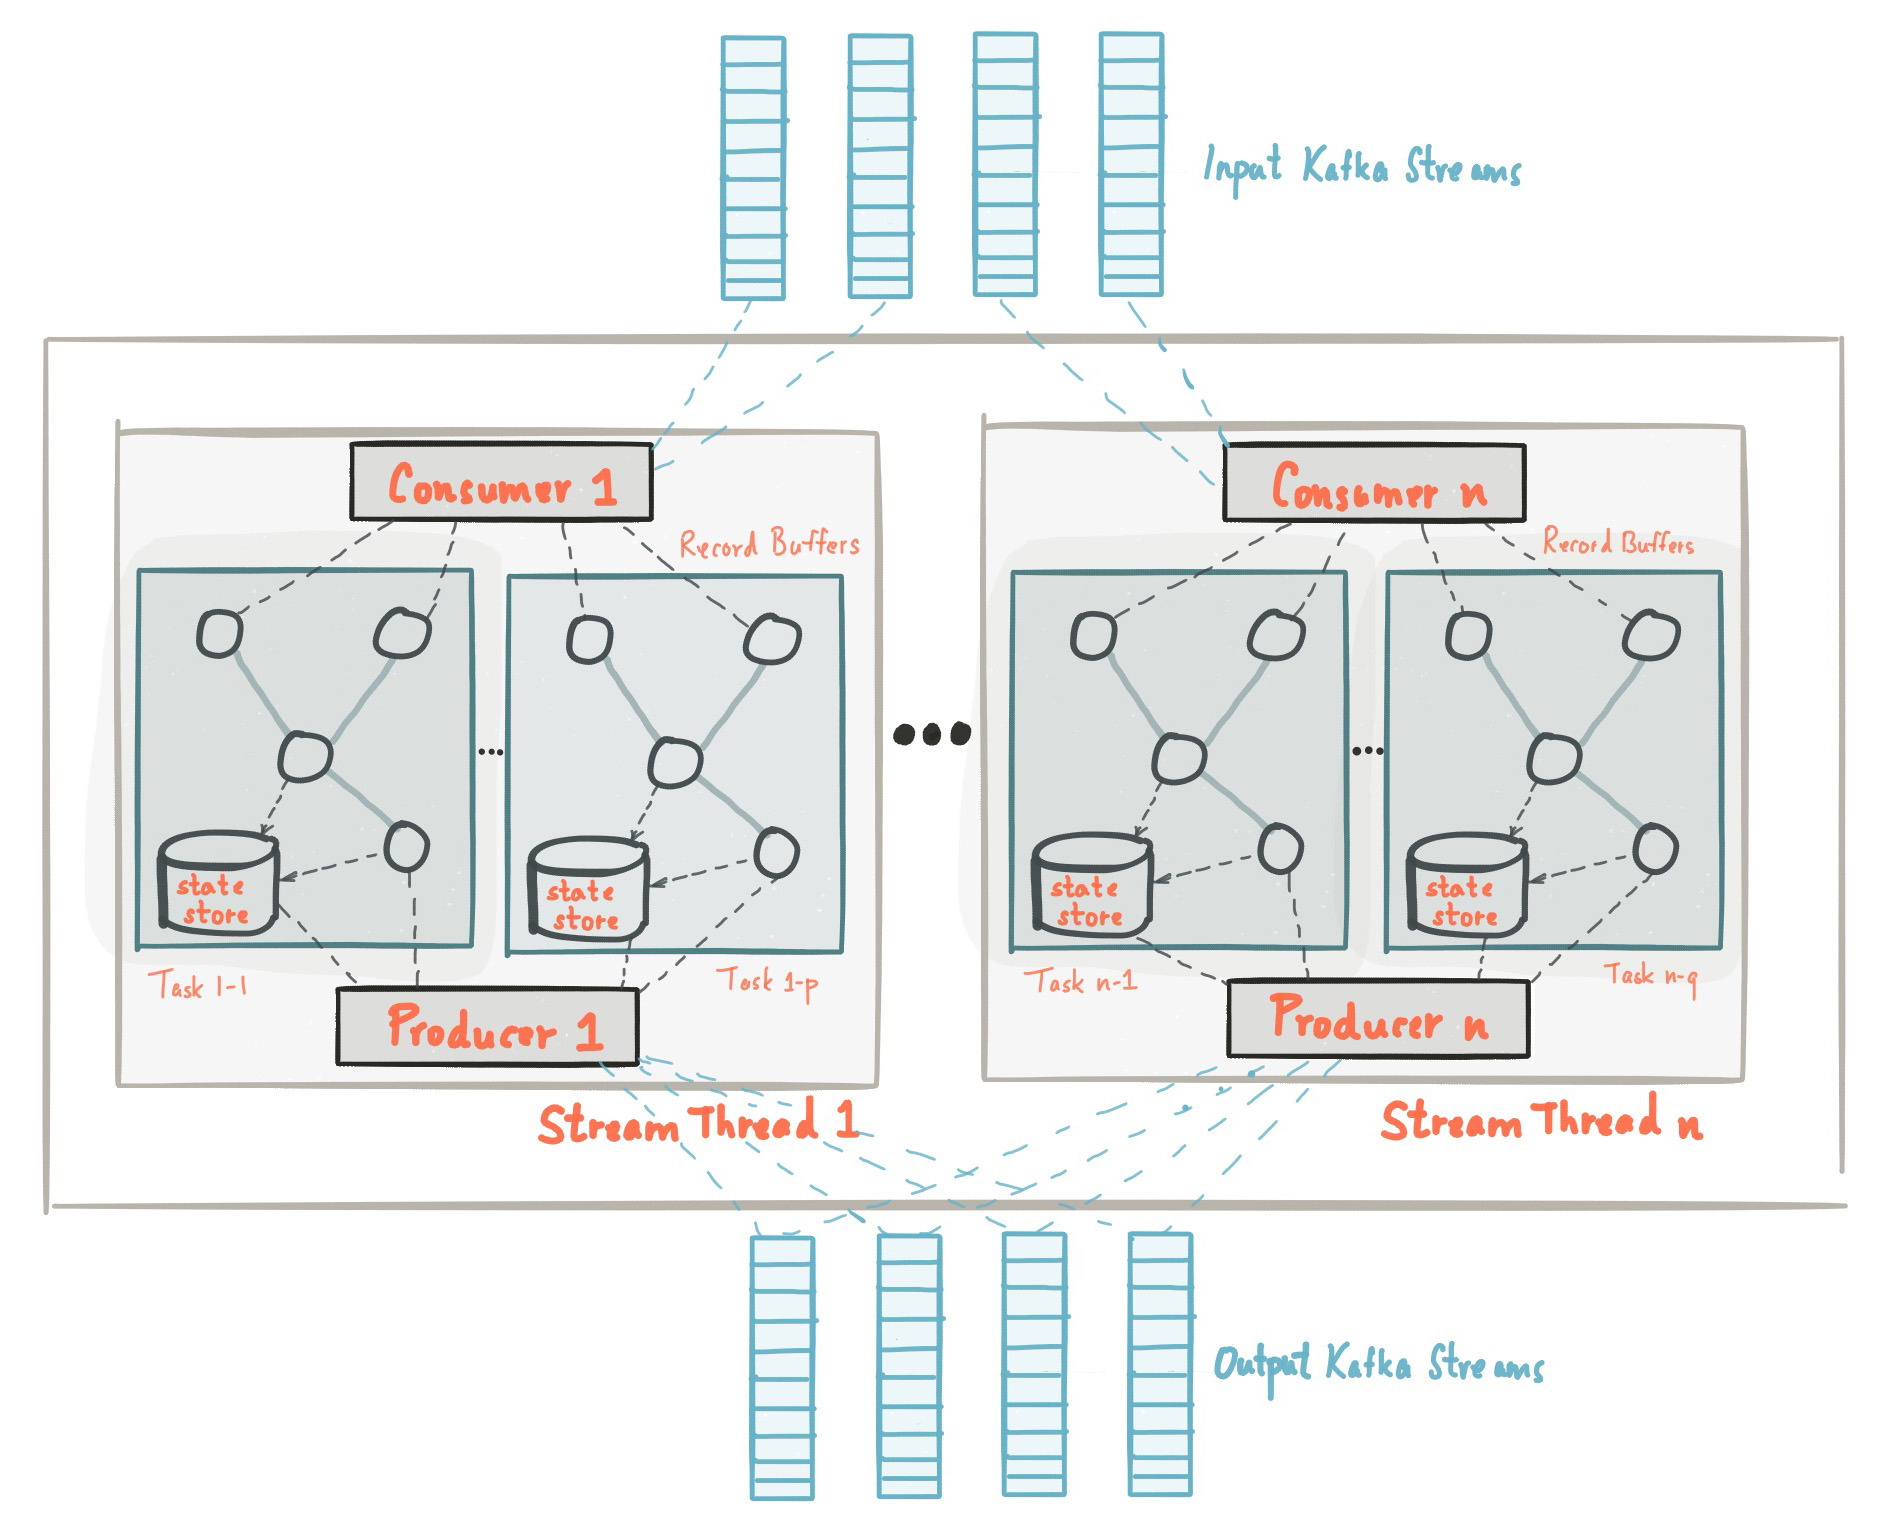
\includegraphics[width=0.7\linewidth]{figs/kafka-streams-overview-v26.jpg}}
\caption{Kafka Streams architecture overview. Producers write events to topics, consumers subscribe and process events, and Kafka Streams provides higher-level stream processing functions. Source: Apache Kafka Documentation \citep{kafkaintro2024}.}
\label{fig:kafka_streams_overview}
\end{figure}

\subsection{Apache Flink: Stateful Stream Processing}

Apache Flink \citep{flinkdocs2024} is described as ``a framework and distributed processing engine for stateful computations over unbounded and bounded data streams.'' Flink has been designed to run in all common cluster environments, perform computations at in-memory speed, and scale to any size. Flink integrates with Hadoop YARN, Kubernetes, and can run as a stand-alone cluster.

The Flink architecture is built around four critical concepts \citep{flinkdocs2024}:

\begin{itemize}
    \item \textbf{Continuous processing of streaming data:} Flink applications are composed of streaming dataflows that may be transformed by user-defined operators. These dataflows form directed graphs that start with one or more sources and end in one or more sinks. Applications can consume real-time data from streaming sources (e.g., Kafka, Kinesis) and produce results to various sink systems.
    \item \textbf{Parallel dataflows:} Programs in Flink are inherently parallel and distributed. During execution, a stream has one or more stream partitions, and each operator has one or more operator subtasks. Stream transport between operators can be either \textit{one-to-one} (preserving partitioning and ordering) or \textit{redistributing} (changing partitioning via keyBy, broadcast, or rebalance).
    \item \textbf{Event time processing:} Flink supports using event time timestamps recorded in the data stream, rather than processing time (machine clocks). This enables consistent, accurate analytics regardless of when events are processed, and allows reasoning about when a set of events is complete.
    \item \textbf{Stateful stream processing:} Flink operations can be stateful---how one event is handled can depend on the accumulated effect of all events that came before it. A Flink application running in parallel is effectively a sharded key-value store: each parallel instance of a stateful operator is responsible for handling events for a specific group of keys, with state kept locally for high throughput and low latency.
\end{itemize}

Flink provides exactly-once state consistency through a combination of state snapshots (checkpoints) and stream replay. These snapshots capture the entire state of the distributed pipeline---recording offsets into input queues as well as state throughout the job graph. When a failure occurs, sources are rewound, state is restored, and processing resumes. Flink's asynchronous and incremental checkpointing algorithm ensures minimal impact on processing latencies.

Flink supports both \textit{unbounded streams} (continuous, no defined end, must be continuously processed) and \textit{bounded streams} (batch processing with a defined start and end). Bounded streams are internally processed by algorithms and data structures specifically designed for fixed-size datasets, yielding excellent performance. This makes Flink a unified batch-stream processing engine.

Flink's JobManager coordinates the execution of a Flink job, managing task scheduling, checkpoint coordination, and failure recovery. TaskManagers are worker nodes that execute tasks in parallel within processing slots. Each TaskManager provides a fixed number of processing slots (controlled by taskmanager.numberOfTaskSlots). State is maintained in memory or, if state size exceeds available memory, in access-efficient on-disk data structures (RocksDB state backend). Applications can leverage virtually unlimited amounts of CPUs, main memory, disk, and network I/O, with Flink reported to process multiple trillions of events per day and maintain multiple terabytes of state in production deployments.

The distinction between batch and streaming DQ is fundamental. In batch processing, all records are available before validation, enabling complete statistical analysis. In streaming, records arrive incrementally, requiring online algorithms that update statistics incrementally and validate records with minimal latency.


% ================================================
% 1.3 MLOps: Machine Learning Operations
% ================================================
\section{MLOps: Machine Learning Operations}

MLOps (Machine Learning Operations) is an ML engineering culture and practice that aims at unifying ML system development (Dev) and ML system operation (Ops) \citep{googlemlops2024}. Practicing MLOps means advocating for automation and monitoring at all steps of ML system construction, including integration, testing, releasing, deployment, and infrastructure management. Only a small fraction of a real-world ML system is composed of the ML code -- the required surrounding elements are vast and complex.

The essential MLOps system components are:

\begin{itemize}
    \item \textbf{Configuration:} Model hyperparameters, feature engineering parameters, pipeline configurations.
    \item \textbf{Automation:} CI/CD pipelines for training and serving.
    \item \textbf{Data Collection:} Continuous ingestion of training and validation data.
    \item \textbf{Data Verification:} Automated validation of data quality and schema.
    \item \textbf{Testing and Debugging:} Unit tests for code, validation tests for data and models.
    \item \textbf{Resource Management:} Compute infrastructure for training and inference.
    \item \textbf{Model Analysis:} Evaluation metrics, fairness metrics, behavioral testing.
    \item \textbf{Process and Metadata Management:} Experiment tracking, model versioning, lineage.
    \item \textbf{Serving Infrastructure:} Model deployment, A/B testing, canary rollouts.
    \item \textbf{Monitoring:} Production model performance, data drift, concept drift detection.
\end{itemize}

MLflow \citep{mlflow2024} is the industry-standard open-source platform for MLOps, providing experiment tracking, model versioning, model registry, and serving capabilities. CA-DQStream uses MLflow for experiment tracking and model lifecycle management.

\subsection{MLOps Maturity Levels}

The MLOps maturity model \citep{googlemlops2024} defines three progressive levels:

\begin{itemize}
    \item \textbf{Level 0 (Manual):} Entire ML pipeline is manual. Data scientists train models in notebooks, hand off to engineers for deployment. No CI/CD, no continuous training (CT). Suitable for systems where the model rarely changes.
    \item \textbf{Level 1 (Automated ML Pipeline):} The ML pipeline is automated so that it continuously trains models in production. CT is enabled via automated data and model validation, triggered by scheduled jobs or data/model changes. Still typically manual for deploying model updates.
    \item \textbf{Level 2 (Automated ML with CI/CD):} The ML pipeline is automated with a robust CI/CD system. Data scientists can rapidly explore new features, algorithms, and model architectures. The system automatically builds, tests, and deploys new pipeline components. This level enables rapid iteration and production-grade reliability.
\end{itemize}

CA-DQStream targets MLOps Level 2, with automated ML training triggered by ADWIN drift detection, CI/CD via containerized deployment, experiment tracking with MLflow, and continuous monitoring of model performance in production.

% ================================================
% 1.4 DAMA-DMBOK Data Quality Dimensions
% ================================================
\section{DAMA-DMBOK Data Quality Dimensions}

The Data Management Association (DAMA) and the Data Management Body of Knowledge (DMBOK) define six core data quality dimensions that guide DQ assessment \citep{dama2017dmbok}:

\begin{enumerate}
    \item \textbf{Completeness:} The degree to which data is not missing. Measured by the proportion of NULL or blank values in required fields.
    \item \textbf{Validity:} Data conforms to defined syntax and semantic rules. For example, fare amounts must be non-negative.
    \item \textbf{Accuracy:} The degree to which data reflects the real-world phenomenon it describes. Detected through outlier analysis and cross-validation.
    \item \textbf{Consistency:} Freedom from contradiction within or across datasets. Cross-feature consistency rules detect values that contradict each other (e.g., cash payments should have zero tip).
    \item \textbf{Timeliness:} Data is current enough for its intended use. Measured by event-time vs. processing-time lag.
    \item \textbf{Uniqueness:} No duplicate records exist. Detected through key-based deduplication.
\end{enumerate}

CA-DQStream addresses all six dimensions through its layered architecture, as detailed in Chapter 3.

% ================================================
% 1.5 Related Works
% ================================================
\section{Related Works}

\subsection{Context-Aware Data Quality}

\textbf{Context Modeling:} Prior work on context-aware DQ includes systematic literature reviews \citep{contextdq2022} that identify context as a critical but under-defined concept in DQ management. While practitioners intuitively understand that data quality thresholds vary by context (e.g., ``a \$50 fare is high \emph{for a standard trip} but normal \emph{for an airport trip}''), formal mathematical models for context-aware thresholding in streaming systems are scarce.

\textbf{Context Dimensions:} Research on multi-dimensional context modeling in data quality has explored spatial context (location-dependent thresholds), temporal context (time-of-day, seasonality), and categorical context (entity types, transaction categories). However, these approaches typically use \textbf{manual threshold specification} per context cell or \textbf{separate models per context}, leading to scalability and maintenance challenges. CA-DQStream's 4D threshold matrix ($7 \times 4 \times 3 \times 7 = 588$ cells) with automatic baseline computation and fallback strategy addresses these limitations.

\textbf{Threshold Adaptation:} Traditional DQ systems use fixed global thresholds that require manual tuning and become stale as data distributions evolve. Recent work on adaptive thresholding has explored percentile-based methods and statistical process control, but these approaches still collapse heterogeneous data into a single threshold. CA-DQStream's contribution is the integration of \textbf{multi-dimensional context with automated threshold computation} ($\mu_{\text{cell}} + 2\sigma_{\text{cell}}$) and intelligent fallback for sparse cells.

\textbf{Gap:} No existing streaming DQ framework combines (1) multi-dimensional context-aware thresholding, (2) automated threshold computation from training data, and (3) drift-aware threshold recalibration. CA-DQStream fills this gap with the 4D context-aware threshold matrix that reduces FPR from 38.7\% (global threshold) to 4.2\% (context-aware) --- a 9.2$\times$ improvement validated on 72M records.

\subsection{Rendezvous and Fork-Join Patterns}

\textbf{Stream Processing Architectures:} Traditional streaming data quality pipelines use \textbf{linear (sequential) architectures} where records flow through validation stages in series: Schema $\to$ Rules $\to$ ML $\to$ Sink. This design suffers from latency accumulation (each stage adds delay) and cascading failure (downstream failure blocks upstream).

\textbf{Fork-Join Parallelism:} The \textbf{Rendezvous pattern} (also known as fork-join or branch-and-merge) has been studied in distributed systems and stream processing for workload parallelization. The pattern splits a stream into parallel branches, processes them independently, and merges results at a synchronization point (rendezvous). Prior work has demonstrated latency reduction and throughput improvement in general stream processing, but not specifically for data quality validation.

\textbf{Application to DQ:} CA-DQStream applies Rendezvous to data quality validation by forking the stream into a \textbf{Canary branch} (fast rule-based checks) and a \textbf{Complex branch} (slow ML-based scoring). This design enables:
\begin{itemize}
    \item \textbf{Early exit optimization:} 13.5\% of records flagged by Canary bypass Complex entirely
    \item \textbf{Parallel execution:} Clean records are validated by both branches simultaneously
    \item \textbf{Graceful degradation:} System continues with Canary alone if Complex fails
\end{itemize}

Experiment 7 validates latency reduction and throughput improvement through early exit optimization and parallel execution compared to linear pipelines.

\textbf{Gap:} No existing DQ framework uses Rendezvous architecture for validation. Great Expectations, AWS Deequ, Soda Core, and Stream DaQ all use sequential processing. CA-DQStream is the first to demonstrate fork-join parallelism for streaming data quality at scale.

\subsection{Drift Detection}

Concept drift detection is well-studied in machine learning \citep{lu2018learning}. \textbf{ADWIN (Adaptive Windowing)} \citep{bifet2007learning, adwin2025} is a state-of-the-art drift detection algorithm. ADWIN maintains a variable-length window $W$ of recent observations and adaptively splits it into two sub-windows $W_0$ (older) and $W_1$ (newer). At each step, ADWIN tests whether the means of $W_0$ and $W_1$ differ by more than a threshold $\epsilon_{\text{cut}}$:

\begin{equation}
|\hat{\mu}_{W_0} - \hat{\mu}_{W_1}| \geq \epsilon_{\text{cut}}, \quad \text{where } \epsilon_{\text{cut}} = \sqrt{\frac{1}{2m} \cdot \ln \frac{4n}{\delta}}
\end{equation}

where $n = |W|$, $m = \frac{1}{1/|W_0| + 1/|W_1|}$ is the harmonic mean of sub-window sizes, and $\delta$ is the confidence parameter controlling the false positive rate of drift detection. A smaller $\delta$ requires stronger evidence before declaring drift. When the condition holds, $W_0$ is dropped and the window shrinks, adapting to the new distribution.

ADWIN provides the following theoretical guarantees \citep{bifet2007learning}:
\begin{itemize}
    \item \textbf{False positive bound:} $P(\text{false alarm}) \leq \delta$ at any time step
    \item \textbf{Detection delay:} $O\left(\frac{1}{\epsilon^2} \ln \frac{1}{\delta}\right)$ observations after a change of magnitude $\epsilon$
    \item \textbf{Memory:} $O(\log W)$ using exponential histogram compression
\end{itemize}

CA-DQStream applies ADWIN to quality meta-streams (aggregated metrics such as violation\_rate, anomaly\_rate, null\_rate) rather than raw data, enabling self-monitoring of the DQ system itself.

\subsection{ML-Based Anomaly Detection}

\textbf{Isolation Forest} \citep{liu2008isolation} is a production-proven anomaly detection algorithm used at Uber and Grab for real-time anomaly detection. Unlike distance-based methods (LOF, $k$-NN), Isolation Forest explicitly isolates anomalies rather than profiling normal instances.

The algorithm builds an ensemble of $T$ random binary trees (Isolation Trees). Each tree is constructed by recursively selecting a random feature $q$ and a random split value $p$ (uniformly drawn between the feature's min and max), then partitioning data points accordingly. For a data point $\mathbf{x}$, the \textbf{path length} $h(\mathbf{x})$ is the number of edges from the root to the terminating node. The anomaly score is defined as:

\begin{equation}
s(\mathbf{x}, n) = 2^{-\frac{E[h(\mathbf{x})]}{c(n)}}
\end{equation}

where $E[h(\mathbf{x})]$ is the average path length over $T$ trees, and $c(n)$ is a normalization factor based on the average path length of unsuccessful searches in a Binary Search Tree:

\begin{equation}
c(n) = 2 H(n-1) - \frac{2(n-1)}{n}, \quad H(i) = \ln(i) + \gamma \text{ (Euler's constant)}
\end{equation}

The score $s \in [0, 1]$: values close to 1 indicate anomalies (short paths, easily isolated), values close to 0.5 indicate normal points, and values below 0.5 indicate dense normal regions. Training complexity is $O(T \cdot \psi \cdot \log \psi)$ where $\psi$ is the sub-sampling size, making it efficient for large-scale streaming applications.

CA-DQStream integrates Isolation Forest into the Flink processing pipeline to detect multivariate anomalies that business rules cannot express.

% ================================================
% 1.5 Chapter Summary
% ================================================
\section{Chapter Summary}

This chapter reviewed the foundational concepts and related works for this thesis. Streaming data processing with Kafka and Flink provides the infrastructure for real-time DQ monitoring. Existing DQ frameworks (Great Expectations, AWS Deequ, Soda Core, Stream DaQ) provide baseline capabilities but only support basic deterministic rules. The DAMA-DMBOK framework defines six core DQ dimensions, all addressed by CA-DQStream. The next chapter formalizes the research problem, grounded in empirical analysis of the NYC Yellow Taxi dataset, and states the research questions.
